% Chapter 4

\chapter{Experiment One - Information Visualisation of UK Geographic Data} % Main chapter title

\label{Chapter5} % For referencing the chapter elsewhere, use \ref{Chapter1} 

\lhead{Chapter 5. \emph{Experiment One - UK Geographic Data}} % This is for the header on each page - perhaps a shortened title

%----------------------------------------------------------------------------------------

\section{Introduction}

In this chapter, the research model will be exposed to real and large data set which is acquired from the Royal Mail Group UK Limited. The data set is not available freely in the market, however it could be purchased for applications development and research purposes. The visualisation model's all four steps are discussed and how the data set visualisation starting from acquisition and data analysis to data representation and user interaction with option to save and export reports. The postcode experiment is built on the proposed system of a single data set - albeit a large one as contains 27 million data rows, making it an ample size to analyse. However, attached to this data set were several smaller data sets, all of which were to be analysed at the same time as the postcode data. These secondary data sets include information on churches, mosques, supermarkets and schools; all of which will be processed and visualised to create a singular location portal for different users. The process of visualising Royal Postcode Address File (PAF) data set involves various stages of data analysis, representation and interactive layers to bring the visualisation model to life. The process is a step-by-step activity explaining how the data is visualised. The outcome of such a complex and large data and how it could be beneficial to institutions and individuals. 

\section{Acquisition and Data Analysis}

The data sets acquired for this experiment were kindly offered by one of the commercial partners of the Royal Mail. This includes England, Scotland, Northern Ireland, Wales, Jersey, Guernsey and the Isle of Man. The postcode is part of a unique coding system designed for the sorting of mail. Invented and administered by the Royal Mail in 1974, postcodes are abbreviated forms of the whole address, and this system allows the UK to be split into designated delivery points. It was devised as an alphanumeric system, and by 1974 it had adopted national coverage \cite{mail1997postcode}. To help employees and sorting equipment to read and interpret typed or handwritten text on the post, the postcode was designed to make this easier. This is the reason the Royal Mail prefers the postcode to be written on a separate (preferably the last) line of the address. There are various formatting rules surrounding postcodes and layout - and this particularly applies to which letters can or can't be used within it. The reason for this is to cut the confusion caused by letters being mistaken for others or muddled up. For example, an O could be mistaken for a Q, or two of the letter V in succession could be mistaken for a W. Postcodes are also used for a variety of other purposes; some of which include calculation of insurance premiums, the designation of destinations in route planning software and even as the lowest level of aggregation in census enumeration. All of these purposes however, can be achieved through the breakdown and analysis of the data in a particular fashion. The royal mail postcode data has been briefly explained above, however there is further explanation available here \cite{royalmail}. The primary data set for this experiment will be, as mentioned previously, made up of the Royal Mail PAF (Postcode Address File) raw data, which will then be processed using our mashup system and projected onto interactive maps. However, there are a number of complimentary data sets from sources such as Google Maps, Bing, Yahoo and Yell in order to draw a complete picture for our map visualisation. This data includes locations like schools, churches, mosques, hotels, supermarkets, nurseries, surgeries, garages and bus stops, among others. The sub data sets and the Royal Mail data will be processed simultaneously, and the result of this will be more vertical and fully functional data for the final interactive maps. These maps will include multiple layers and allow users to dissect the data to any level.

The first stage of data analysis of this magnitude involves actually acquiring the data. To do this, one will need to follow various procedures and functions to obtain data, whether it is in a structural or a raw format. Data sources could be from various mediums; from a simple disk to a network stream. Quite often the source of the data will be dependent on the nature of the data itself. The Royal Mail PAF data set is quite large and this sort of data will usually only be available through network links or a data disk in its raw format. The data in questions is not available to the general public nor it is free to use. A selection of sample data extracted from the Royal Mail PAF data set. The data fields included are large, which are illustrated in Figures 5.1, 5.2 and 5.3.

\begin{figure}[H]
\centering
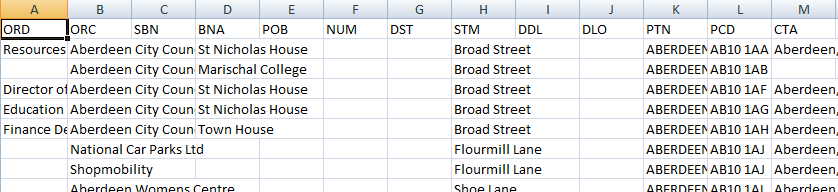
\includegraphics[scale=0.6]{chapter5/raw_date1}
\caption{Royal Mail PAF Data Set Attributes 1}
\end{figure}

\begin{figure}[H]
\centering
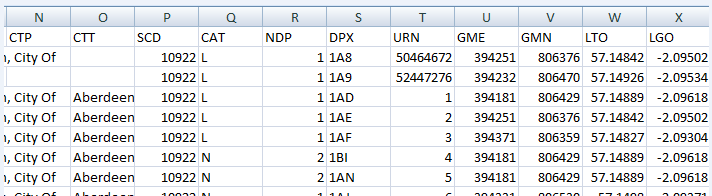
\includegraphics[scale=0.77]{chapter5/raw_date2}
\caption{Royal Mail PAF Data Set Attributes 2}
\end{figure}

\begin{figure}[H]
\centering
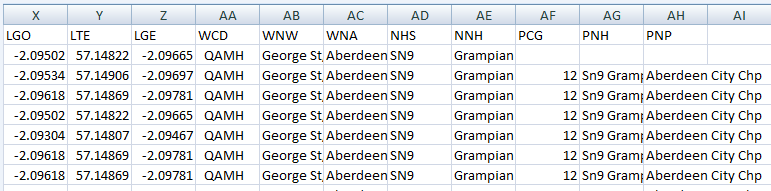
\includegraphics[scale=0.6]{chapter5/raw_date3}
\caption{Royal Mail PAF Data Set Attributes 3}
\end{figure}

The raw data in its full form contains around 36 columns as depicted in Figure 5.4, all representing a different type of data. This is from a postcode, town name to first lines of an address. It also includes more geographically relevant data, such as the UK latitude and longitude, as well as their EU counterparts. In addition to this, they contain more sensitive information about the area described, such as the local government and NHS locality; all of this is a part of the extensive data set. The Royal Mail data set is taken from an extensive database that charts every element of the UK in excruciating detail, using a grid mechanism to define everything about a local area. Using this database, one can identify the names of the local authority, grid points, original and current postal code areas even, the top tiered local government of any area within the UK, no matter how small. A data set of this size is difficult to sift through manually, and equally hard to understand in its raw state. Therefore, need a robust visualisation model to analyse such colossal data.

\begin{figure}[H]
\centering
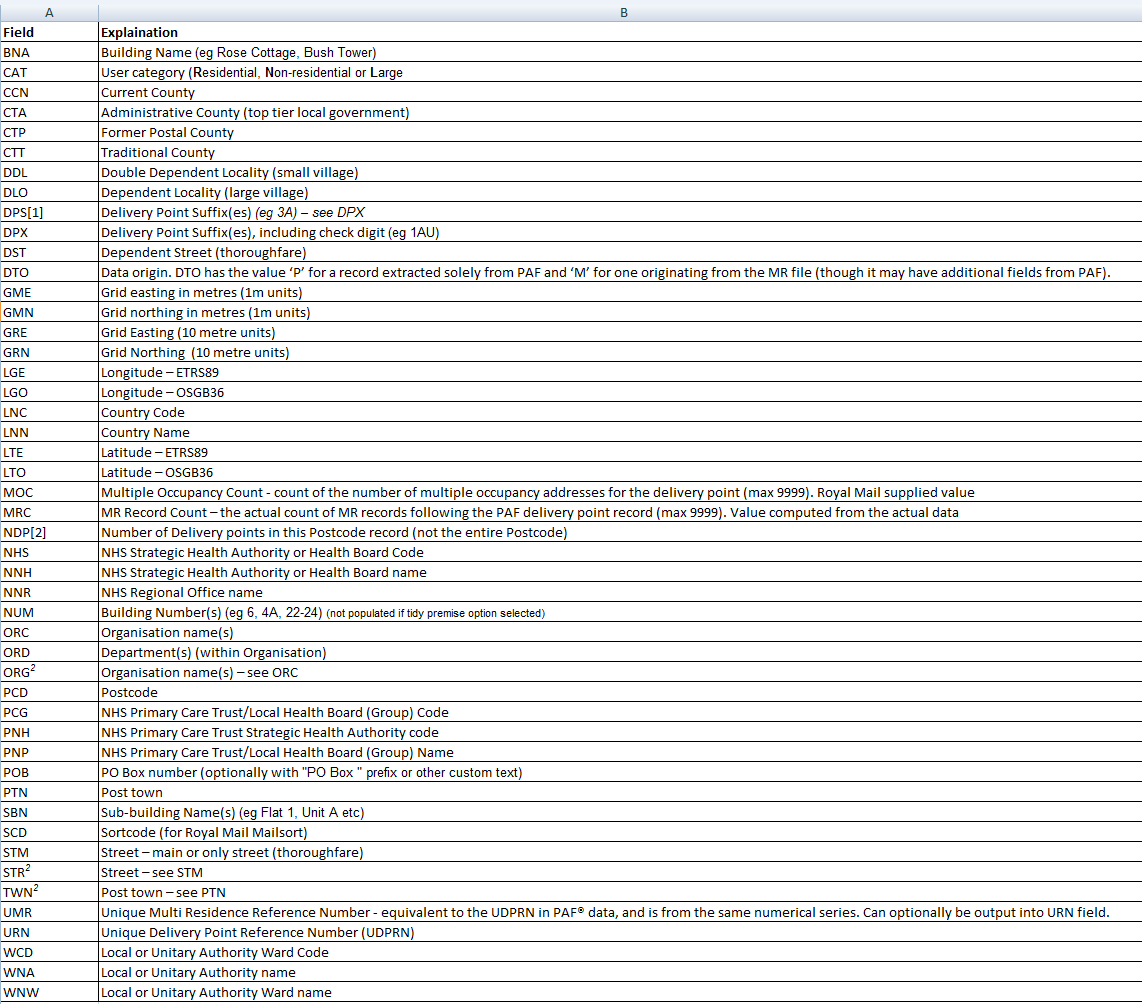
\includegraphics[scale=0.48]{chapter5/psotcode_data_fields}
\caption{Royal Mail PAF Data Set Fields}
\end{figure}
% figures here

The acquired data has been formatted, it is in a compact and readable position to continue. However the data is still not in the perfect state to be able to extract meaning from it, and use this to visualise and produce our map. Small programming codes could help to retrieve such information, it needs to be further refined. There are two more processes that need to be done before the data is ready to be taken to the next step. This will make the data much more compact and meaningful for analysis. As a part of this process, data filtering is essential, as the processing system will remove any duplicated or unwanted information from the data sets. The data is in a much more compact and usable state at this stage, applying filtration methods help to refine it further to make it fit for purpose as demonstrated in Figure 5.5. This also streamlines the data; removing any duplicate rows or columns or anything irrelevant to the analysis. For example, in Figure 5.5 the EU latitude and longitude is not needed for this experiment, so these columns will be removed from the data set during filtration. 

\begin{figure}[H]
\centering
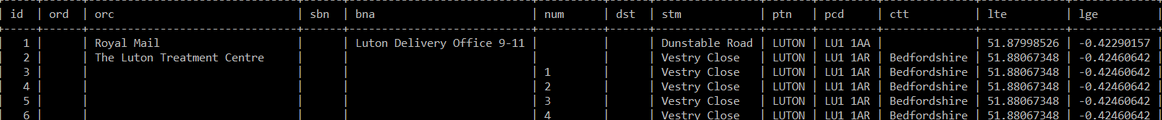
\includegraphics[scale=0.47]{chapter5/parsed1}
\caption{Processed/Parsed Royal Mail PAF Data Set}
\end{figure}

From the original 36 columns of raw data, it is now reduced to a mere 13 columns, as presented in Figure 5.6. The duplicated or unnecessary information and rows are removed from the data set. In this case, information such as flats and sub-houses are taken out, as this is not relevant to the study and will not be used in the visualisation process. Figure 5.6 shows the data before the filtering has been applied. 

\begin{figure}[H]
\centering
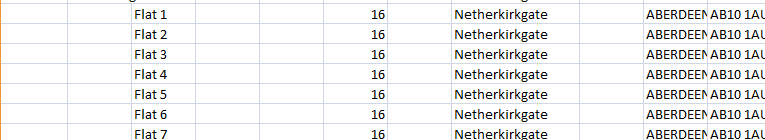
\includegraphics[scale=0.7]{chapter5/flat_filter1}
\caption{Mined / Refined Royal Mail PAF Data Set}
\end{figure}

Through the refinement, the rows above have now been converted into a single row, as illustrated in Figure 5.7. This will make the identification of this area easier and much less cluttered in the final visualisation. The raw data set has repetitive data elements which were filtered at the acquisition and data analysis stage of the information visualisation model. The filtered data is then passed onto the representation layer for visualisation. 

\begin{figure}[H]
\centering
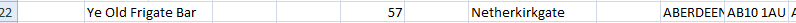
\includegraphics[scale=0.6]{chapter5/flat_filter2}
\caption{Filtered Royal Mail PAF Data Set}
\end{figure}

This process might seem simple and basic, the filter used to apply this process (known as the normalisation and data filter) can be difficult to create and a time consuming process to apply; especially to a data set of this size and complexity. Data mining involves several techniques but the basic premise is that it creates a basic instruction for the computer using a combination of statistics, mathematical analysis and data mining. It starts by shifting the data and applying purely cosmetic changes; for example filtering and removing raw data that is above a certain size or density. This helps remove the information that wasn't relevant or necessary for the desired output. In this experiment, the identified and extracted examples of repetitive postcodes and duplicated rows which are unnecessary was removed. The next section discusses the visualisation model for the acquired data.

\section{Data Representation}

Represent++ is the data representation layer of the proposed visualisation model which allows users to manipulate and understand the data more effectively. Representation of data can have many forms (charts, graphs etc). For this experiment on the UK postcode data, visualisation is done using an interactive map and combine it with data mashup techniques. The data presented to the representation layer is already been processed and analysed in the previous step. The conversion of raw data into a normalised form is then pushed onto the the representation layer where data is visualised with the help of various technologies. The next step in the visualisation plan is utilising the data that has been refined. For this purpose, web maps are the perfect way to display the extracted data, as web maps easily deliver up to date information. If a map is programmed to be generated automatically from a database, it displays new information in real time, without much waiting and further editing. They are also superior to traditional maps, they don't need to be printed, mastered and distributed, are quickly updated and much easier to work with.  A few examples of interactive web mapping in action include:

\begin{itemize}
\item 	A map displaying election results as they are tallied, as soon as they become available from counting.

\item	Maps displaying live traffic updates in almost perfect real time, using data collected by traffic sensor networks. 

\item	A map which shows in detail the current locations of mass transit vehicles (such as busses, trains, ferries or planes). This allows the passengers of the vehicles to  minimize waiting time at stops or stations, and allows to be aware of the delays in service, should there be any. 
\item 	Weather maps used by the media, such as NEXRAD \cite{smith1996intercomparison}
\end{itemize}

Another advantage of using interactive web mapping lies in the cost. The software and hardware used to create map infrastructure for the web is cheap, and web server space and hardware is equally inexpensive, and with many open source tools available for use, it is easy to create professional and fully functional web maps quickly \cite{de2006opengis}.\\

The web maps also give users many more advantages than we perhaps thought of. For example, pushing out and distributing product updates has become a much easier task. This is because web maps distribute data with every single request or load so updates can happen as quickly as a user reloads a page. In more traditional cartography one would need to deal with minor map updates having major ripple effects. If a road name changes or a roundabout is placed, this simple update can be administered in seconds in web maps, but in print it can trigger a reprint, remaster and full redistribution of the media. But one of web maps greatest strengths is also its greatest weaknesses. Because updates are cheaper, easier and faster, it can occur more frequently and even the base product is cheap and quick to create. This is perhaps one of the main reasons many web map's are of astoundingly poor quality; both in symbolisation, content and actual data accuracy. An added bonus for some businesses or organisations interested in this kind of data is that detailed information is now available to discover and combine on a lot of private and personal information of individuals. The details and images of properties and estates of private individuals are now accessible to the general public in high resolution through the web mapping tools. Web maps also allow for complete personalisation. Through the utilisation of user profiles, personal filters, styling and symbolisation anyone can spawn, configure and design their own maps from scratch, providing their chosen platform and mapping system supports personalisation. This personalisation even reaches into the realms of accessibility, and can be used to solve a series of problems. Users can personalise various maps, storing their favourite colours and patterns to identify areas while avoiding colour combinations users can't easily distinguish due to medical or accessibility reasons (e.g. colour blindness) \cite{ware2013information}. Figure 5.8 highlight an interactive map, which was created by processing data through our data mashup system. Using this the Royal Mail postcode data will be visualised. This map shows the United Kingdom as a general space, and separates it into basic geographical locations. 
 
\begin{figure}
\centering
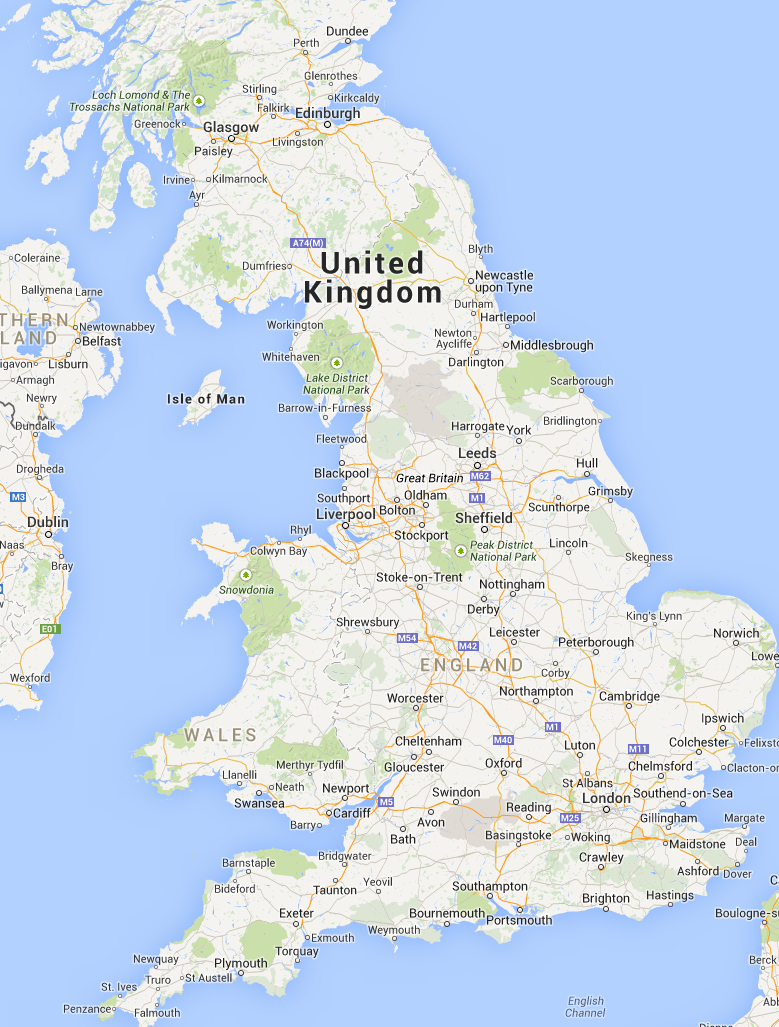
\includegraphics[scale=0.7]{chapter5/web_map1}
\caption{Interactive UK Map Generated}
\end{figure}

Figure 5.9 shows a section of the map segregated by postal regions using the Royal Mail postcode data that have been refined It has been visualised on a fully interactive map, and using web intelligent agents users can read data from the database and feed it back in real time.

\begin{figure}
\centering
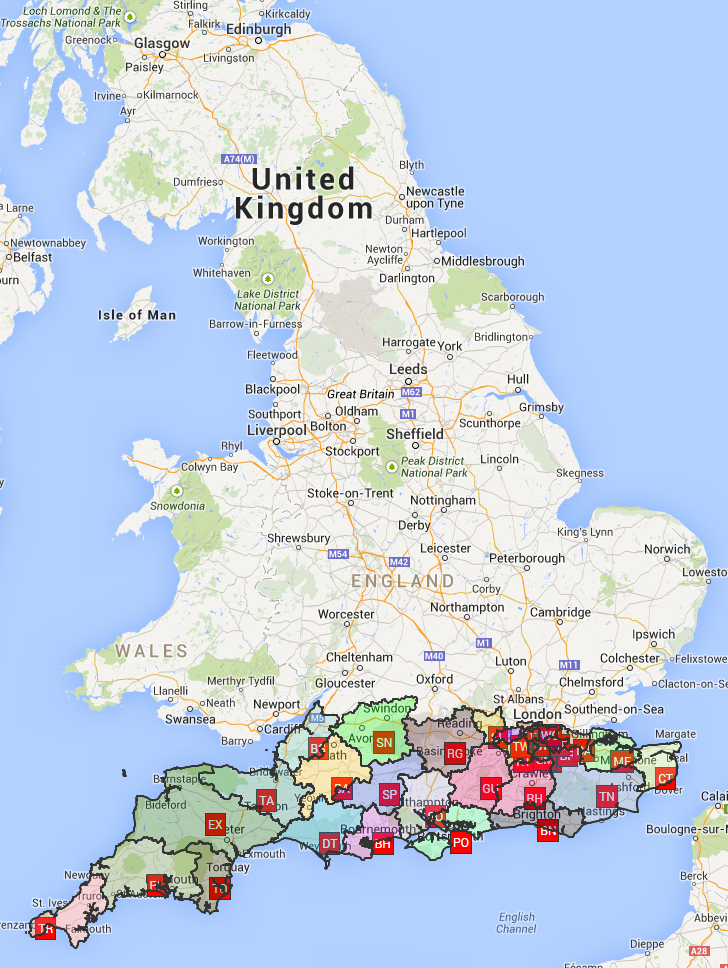
\includegraphics[scale=0.75]{chapter5/web_map2}
\caption{Extracted Postcodes are Visualised with Tags}
\end{figure}	
 
Figure 5.10 demonstrates, data at its next development phase. All of the postcodes are collected from the data set for the entirety of the UK, and have been used to visualise postal boundaries. Red blocks are used to act as tags for each postcode shown, and coloured lines to signify borders. This data can be utilised in several different ways; for example, population density, economic growth, living standards and various other social attributes could be visually portrayed for public and readers. 
 
\begin{figure}
\centering
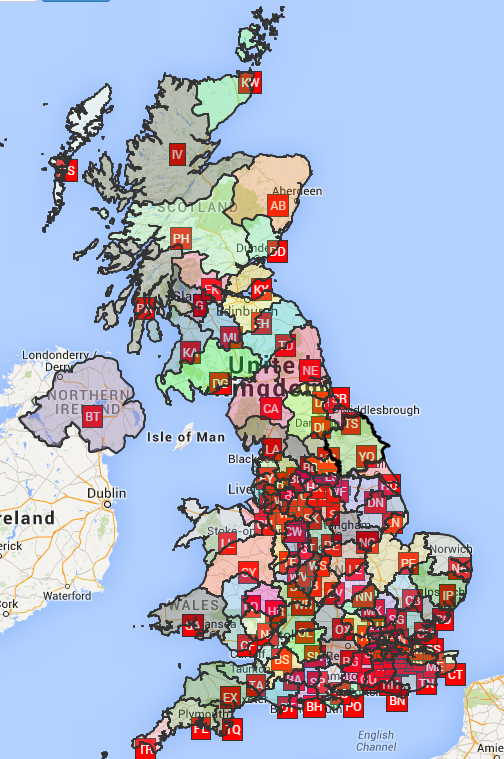
\includegraphics[scale=0.9]{chapter5/web_map3}
\caption{Postcodes are Categorised and Visualised with Animation}
\end{figure}

Once all of the information is collected, users can look closer and dissect it further, Figure 5.11 in the selection is a close up of the Nottingham area. It illustrates a highlighted area in a colour of user's choice for each individual post code area.
 
\begin{figure}
\centering
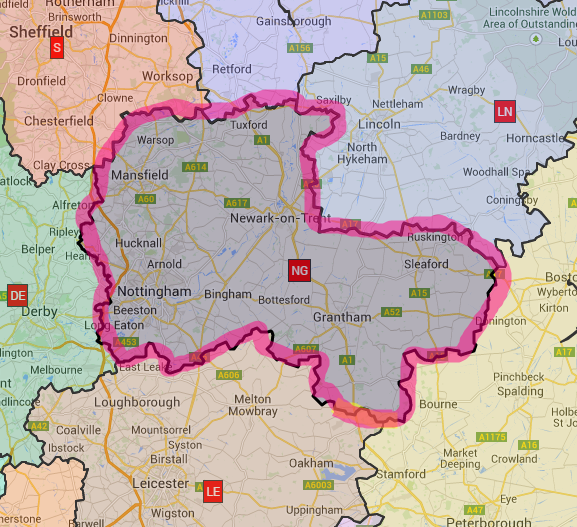
\includegraphics[scale=0.8]{chapter5/web_map4}
\caption{Postcodes Shown with Boundary Markers}
\end{figure} 

Figure 5.12, schools and colleges are shown along with the Royal Mail postcode data illustrated on the map with postcode boundaries. Thus making very easy for the users to understand which colleges or schools fall under what postcodes, these maps are further discussed in chapter 7.

%figure 12
\begin{figure}
\centering
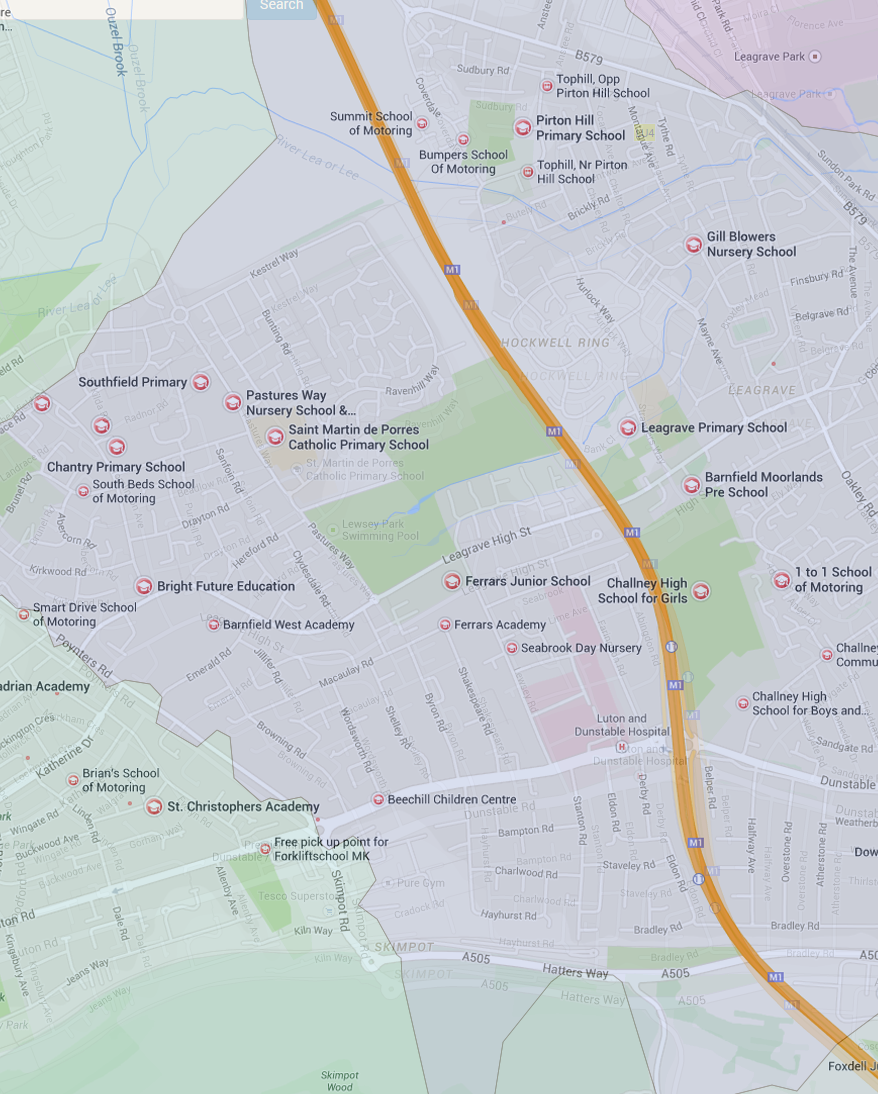
\includegraphics[scale=0.47]{chapter5/schools_map}
\caption{Postcodes Shown with Boundary Markers With Colleges/Schools}
\end{figure} 

The data was retrieved from the database which was initially refined and structured in the acquisition and data analysis layer. This layer have retrieved information from the database through web intelligent(PHP functions) and visualised on an interactive map, where postcodes information is shown in various types. The first or the default screen of the system in this layer shown full UK map with postcode classification and categorisation. The end user can quickly see where a postcode starting with two characters located on what area of the country. The view is further explored through input or zooming in from the user to see further information on a specific area, which then gives additional sub postcode geographic areas distinguished with different colours and surrounded by the boundaries of the postcodes. Sub postcode is additional division of the postcode. The third and final view of the map gives complete list of the postcode in the specified or user selected areas, giving precise information which streets falls under a particular postcode. The postcode map could be an education tool for people from all round the society, with creating knowledge and awareness about UK geography and specially encouraging people to understand complex postcode system with an ease. The next section discuss how the user interact with the data and the web map system.

\section{Interaction }

The next phase of the experiment is about the user and system interaction, which involves adding a new layer onto the interactive map. This new layer of visualisation model acts as a system, and this is utilised to help users gain the ability to interact with the data. This is what transforms the map from a reactive model into an interactive one. Without it, users can't explore the data and gain a deeper understanding. Interacting with data requires digging deeper into the sub levels of the data, finding the hidden gems of information that are not visible at the higher level view. For example, if a user is to select a postcode from those listed in the data or tagged on the map, users can zoom into the interactive map to study it in more detail. When in this view, the user can now see additional sub categories that were not available in the initial view in this case the sub-postcodes that are depicted in Figure 5.13. These are identified with yellow tags, and more information is displayed the further on the map as the user descends further.

\begin{figure}
\centering
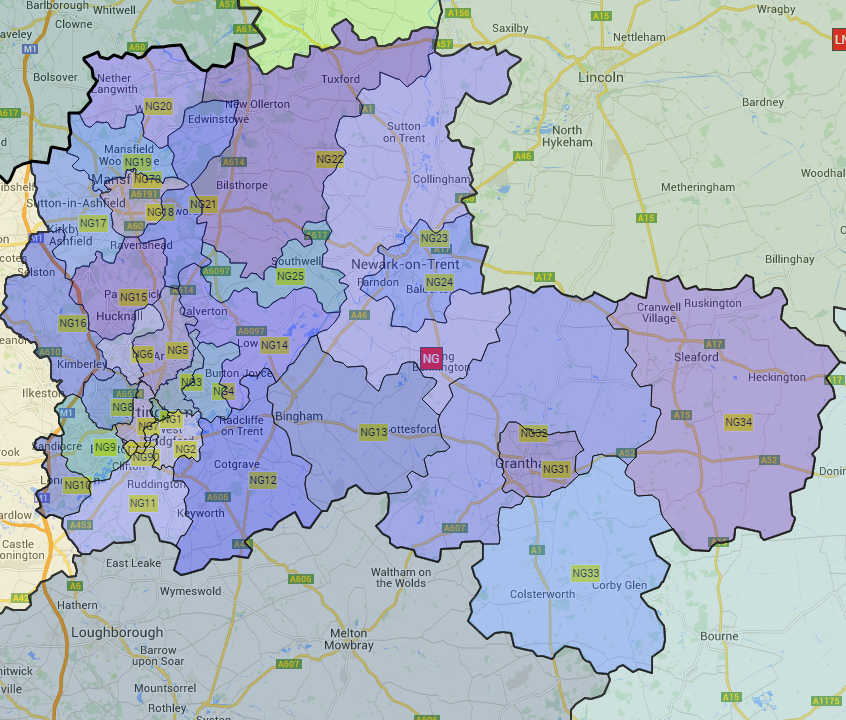
\includegraphics[scale=0.65]{chapter5/web_map5}
\caption{Sub Categorisation of Postcodes Shown with Boundary Markers & Colours}
\end{figure} 

These little sub categories give even more information to the user and the system understands and compensates for that. The system used to create this interactive map is incredibly intelligent, and the new sub categories that are available are now marked with their own tags and boundaries. These are all in different colours with corresponding tags, while still remaining different from the upper levels of distinction. In this new level of interaction, a user can quickly and easily see where NG33 lies on this map. NG33 is sub postcode located in the city of Nottingham as demonstrated in Figure 5.14.

\begin{figure}
\centering
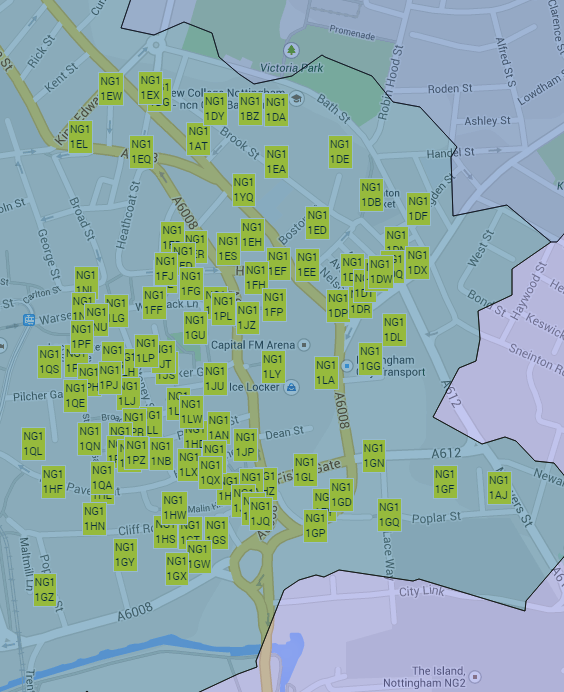
\includegraphics[scale=0.8]{chapter5/web_map6}
\caption{Detailed Postcodes Visualisation with Boundary Markers & Colours}
\end{figure} 

The information could be drilled down further and further, into more detail by continuing to refine the data, searching or interacting with the system. As it is demonstrated above, the further user dig, the more detailed information about the postcode can be shown on the map. It is highlighted clearly where each postcode is located on the map, and if users choose to investigate further they could see the street names belonging to each postcode at each address.

The model has shown the capability of possessing a large, bulky set of data which was quite challenging to understand or manage to having a fully visualised version that is streamlined and easy to read. This has involved many different processes, streamlining, filtration, data mining and parsing before it has arrived at this stage and without those key processes the data would still be almost unusable. This practice can be applied to any form of data set on any subject, and can be used to convert masses of data into simple visualisation forms. By visualising the data in this way, users are able to discern more than one would be able to at face value. The result of the process doesn't have to be a map either there are various other visualisation styles available that can be used to give decision makers key insights about business transactions and customers. These different visualisation styles are highlighted in experiment two. Exporting reports and data storage is discussed in the next section.

\section{History}

The users are given option to export reports into JPEG, GIF, PNG and PDFS. The system produces high resolution images and screen extractions for external usage. The map available to user at the interact++ layer also has the feature to copy link of the generated map along with tags highlighted for points of interest such schools, colleges, churches, mosques or supermarkets. This tool becomes a quality asset for users who are keen to learn UK geography through the postcode perspective or based on the location attributes. The reports and maps are also available to web services which could easily be embedded into any other application. 

\section{Summary}

A complex data set has been processed and analysed and then presented into a visualised form thus exploring data at a different angle. The base data set has been experimented with additional data set for the added value features. The visualisation model and its four stages are explained individually supported by figures and screen shots from the application. In the next chapter, a different type of data set has been analysed. The data set in chapter 6 is a business transactional data set. The same four stages of visualisation are followed data representation and interaction with user. 




